This chapter introduces related work that was used in the development of this project. First, we introduce diffusion models in  \cref{sec:diffusion_models}.

\section{Diffusion Models} \label{sec:diffusion_models}

Diffusion models are machine learning systems trained to denoise random gaussian noise step by step, to get to a sample image. Neural networks are trained to predict a way to slightly denoise the picture in each step. As we can see in \cref{fig:diffusion_process}, after a certain number of steps, a sample is obtained.

\begin{figure}[ht]
    \centering
    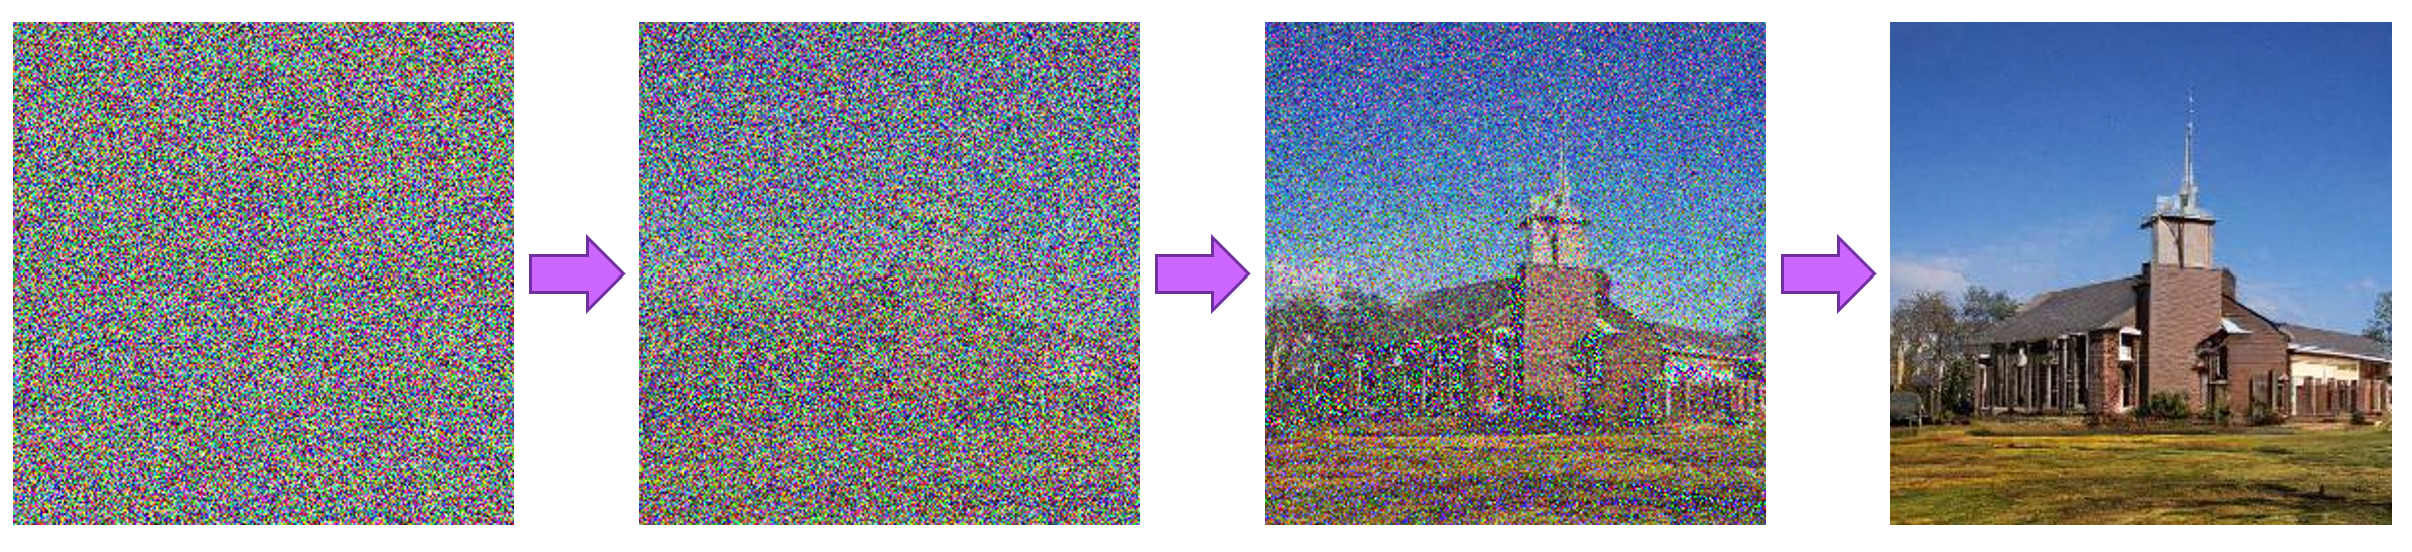
\includegraphics[width=\linewidth]{images/diffusion-process.png}
    \caption{In the diffusion process random images are denoised in multiple steps to get a sample image. Source: \url{https://github.com/huggingface/notebooks/blob/main/diffusers/diffusers_intro.ipynb}}
    \label{fig:diffusion_process}
\end{figure}

Diffusion models have obtained SOTA results on image generation. However, one downside of diffusion models is that the reverse denoising process is slow. In addition, these models consume a lot of memory because they work in pixel space. Therefore, it is challenging to train these models and also to use them for inference.

Consequently, most of the recent diffusion models, e.g. DALLE-2 \cite{ramesh2022hierarchical} and IMAGEN \cite{saharia2022photorealistic}, are unfortunately not accessible to the community. The most popular exception is Stable Diffusion \cite{rombach2021highresolution}, which has been open sourced and can be used on a single GPU.

\subsection{Stable Diffusion}

Stable Diffusion is based on a type of diffusion model called Latent Diffusion \cite{rombach2021highresolution}. Latent diffusion reduces the memory and compute complexity by applying the diffusion process over a lower dimensional latent space. There are three main components in latent diffusion: an autoencoder (VAE), a U-Net and a text-encoder (CLIP).

\paragraph{The autoencoder (VAE) \cite{kingma2013auto}.} The VAE has two parts, an encoder and a decoder, as we can see in \cref{fig:vae}. During latent diffusion training, the encoder maps the images to a latent space for the forward diffusion process, which applies more noise at each step. During inference, the decoder maps the latents generated by the reverse diffusion process back to the images. The encoder and decoder are trained jointly to minimize the reconstruction error.

\begin{figure}[ht]
    \centering
    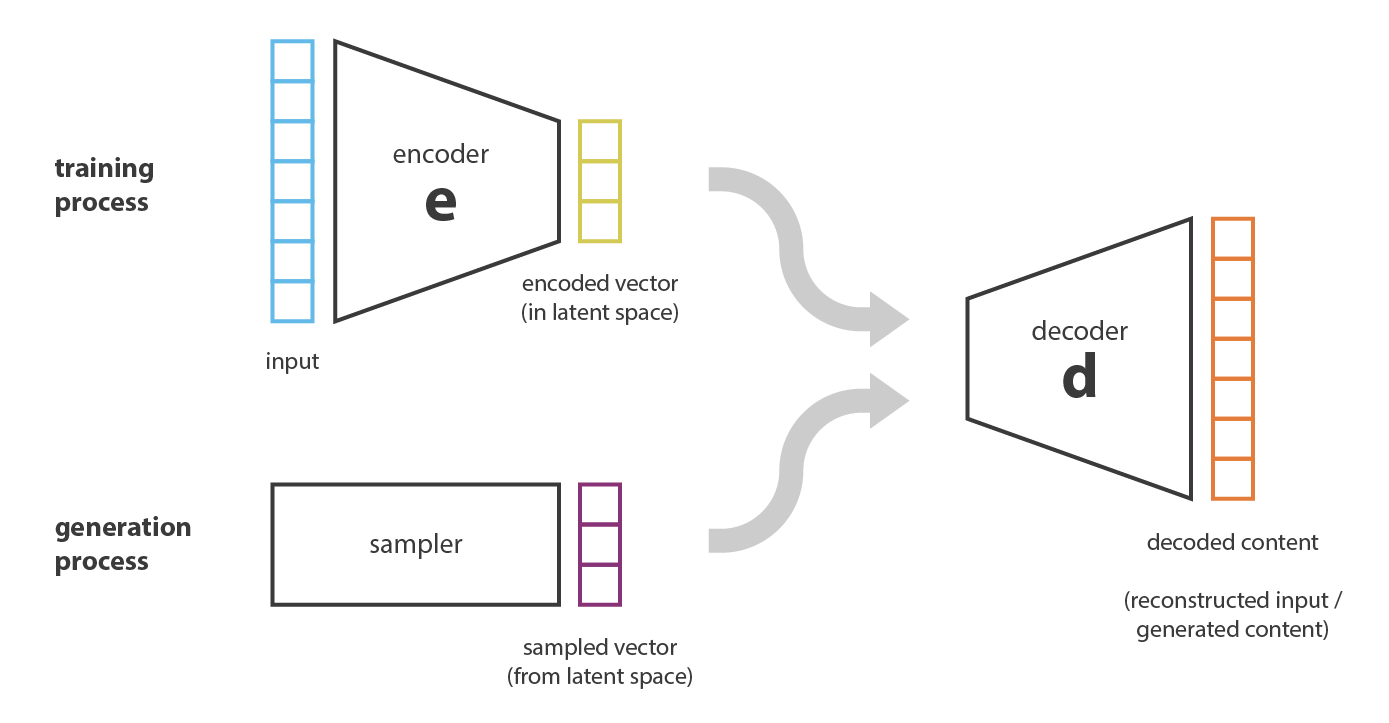
\includegraphics[width=\linewidth]{images/vae.png}
    \caption{Variational Autoencoder (VAE) training and generation processes. Source: \url{https://towardsdatascience.com/understanding-variational-autoencoders-vaes-f70510919f73}}
    \label{fig:vae}
\end{figure}

\paragraph{The U-Net \cite{ronneberger2015u}.} The U-Net also has an encoder part and a decoder part, as shown in \cref{fig:unet_model}. The encoder has several ResNet blocks which half the image size by 2. The decoder does the opposite process to upsample the image to the initial size. The U-Net outputs the noise residual which can be used to compute the denoised image representation. To prevent the U-Net from losing important information while downsampling, shortcut connections are usually added from the downsample path to the corresponding layers in the upsample path. Moreover, the output of the stable diffusion U-Net is conditioned on text-embeddings via cross-attention layers.

\begin{figure}[ht]
    \centering
    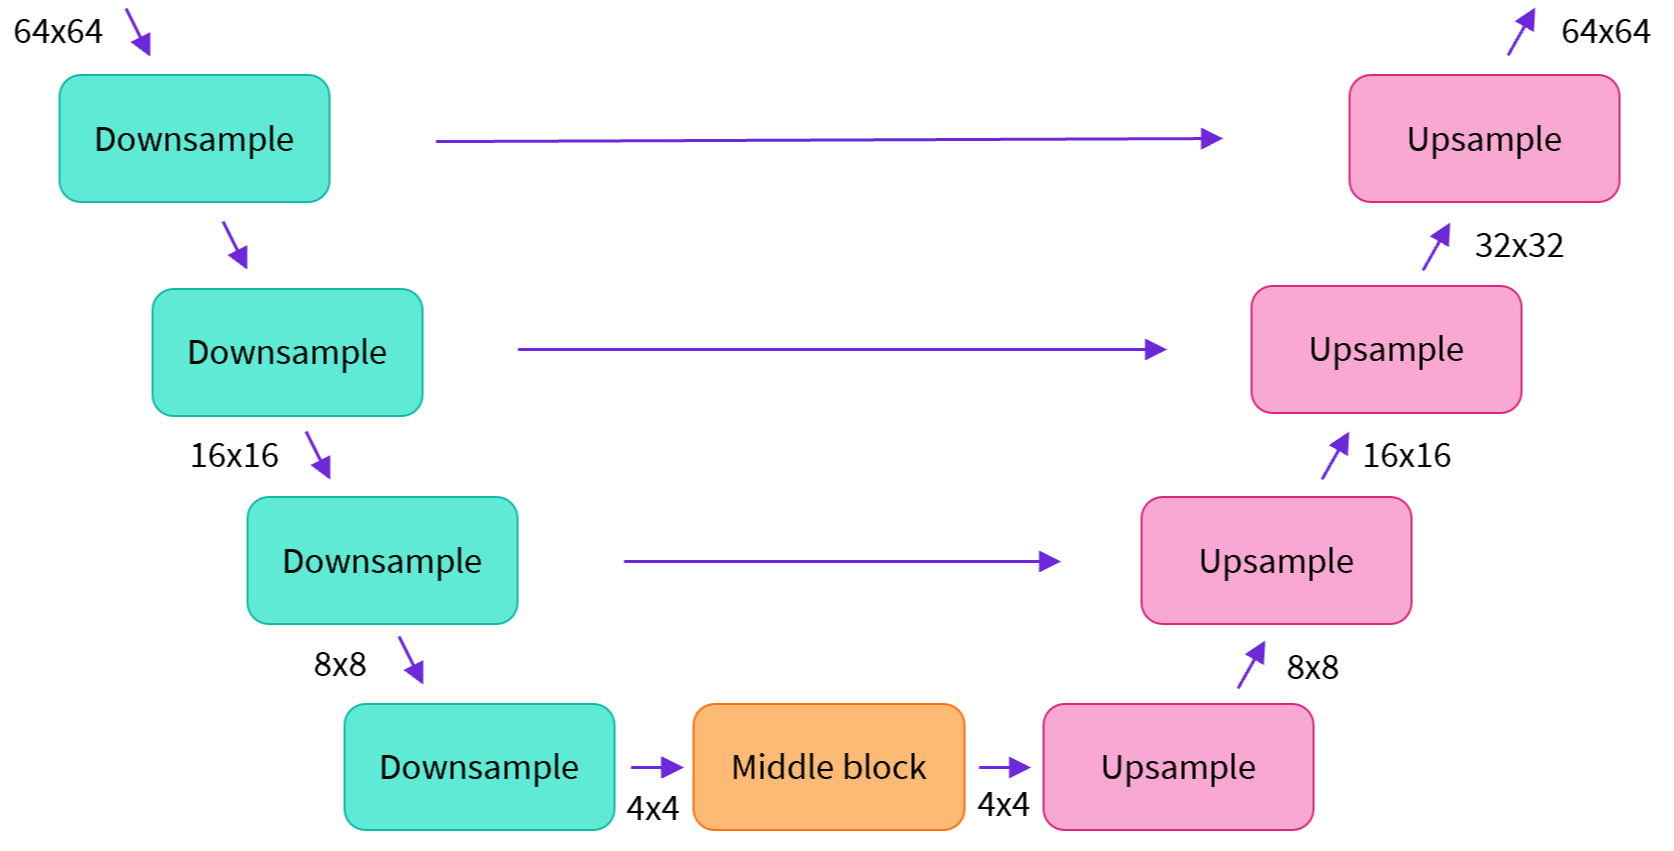
\includegraphics[width=\linewidth]{images/unet-model.png}
    \caption{The architecture of the U-Net model. Source: \url{https://github.com/huggingface/notebooks/blob/main/diffusers/diffusers_intro.ipynb}}
    \label{fig:unet_model}
\end{figure}

\paragraph{The text-encoder (CLIP) \cite{radford2021clip}.} The text-encoder transforms the input prompt into an embedding for the U-Net. Stable Diffusion does not train the text-encoder during training and uses an already trained CLIP text encoder, which is shown in \cref{fig:clip}.

\begin{figure}[ht]
    \centering
    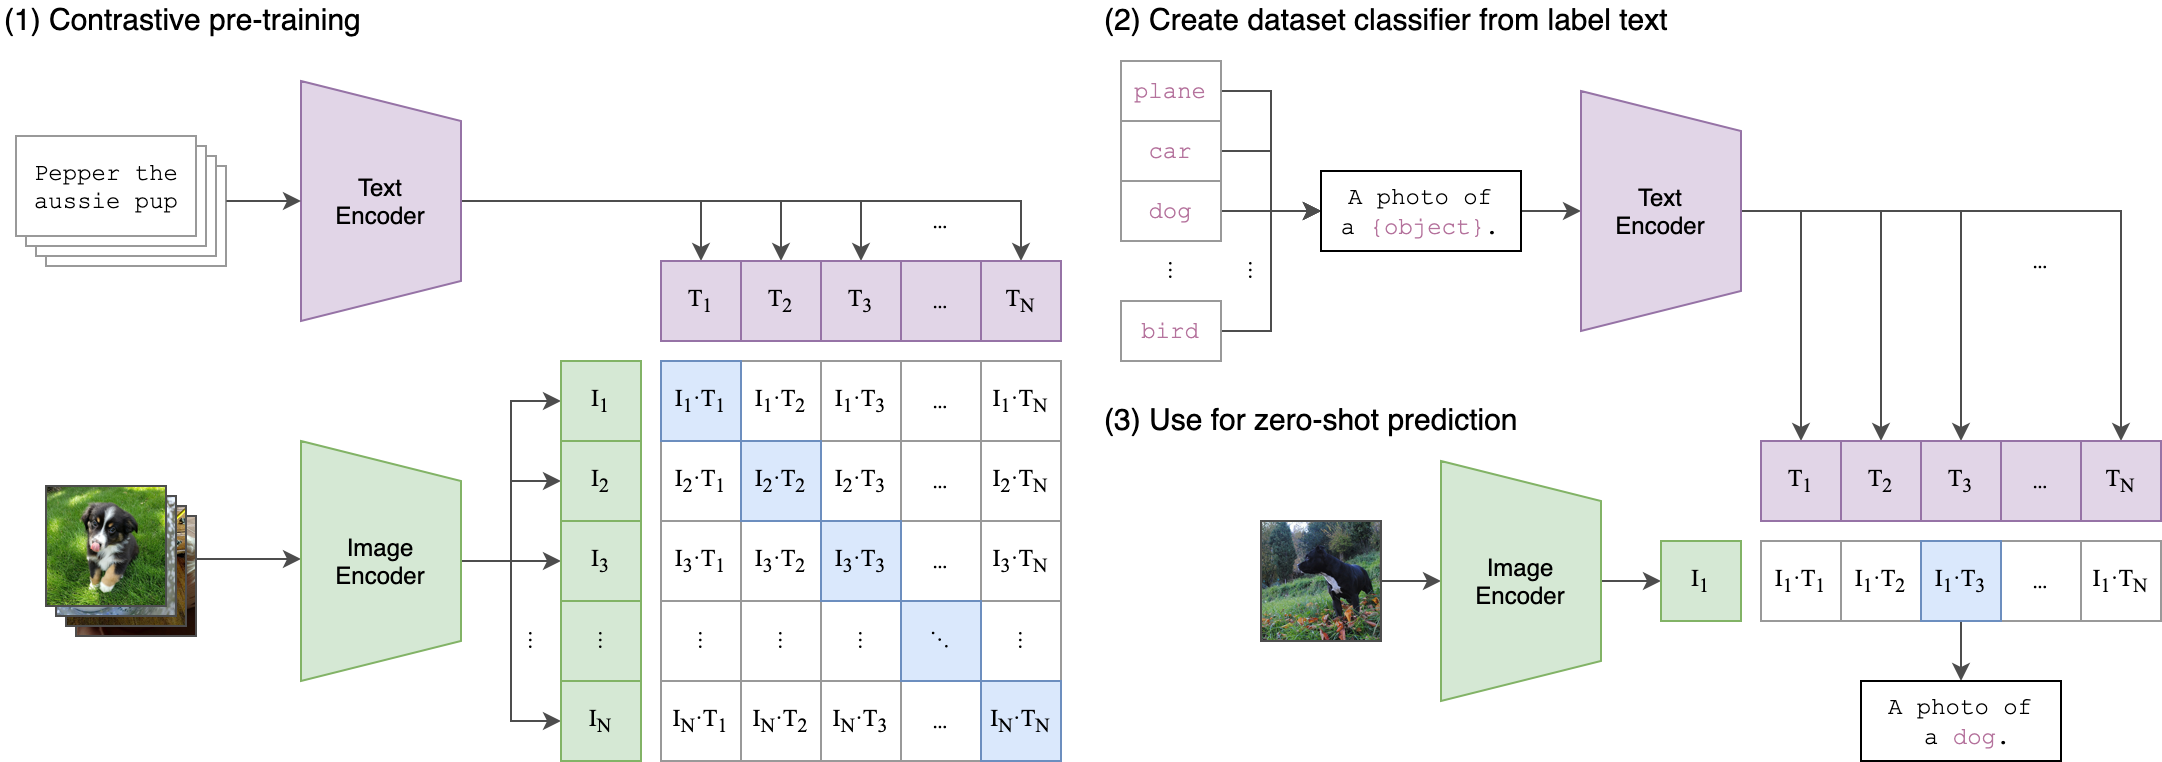
\includegraphics[width=\linewidth]{images/clip.png}
    \caption{CLIP model architecture. Source: \url{https://github.com/openai/CLIP}}
    \label{fig:clip}
\end{figure}

With the previous components we nearly have the full Stable Diffusion inference architecture \cref{fig:stable_diffusion}. The stable diffusion model takes a latent seed and a text prompt as input. The latent seed is  used to generate initial random latents. The output of the U-Net is used to compute a denoised image representation with a scheduler algorithm. This process is repeated many to get better representations in each iteration. Finally, the latent image representation is decoded by the VAE decoder.

\begin{figure}[ht]
    \centering
    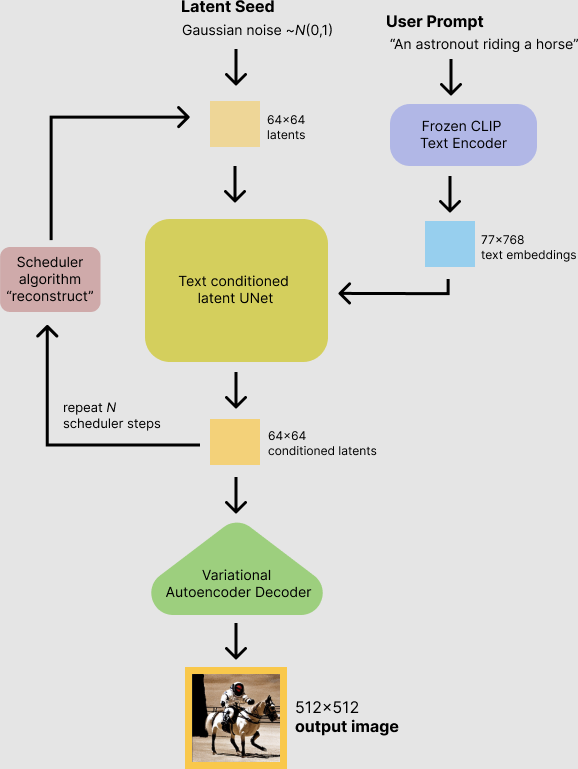
\includegraphics[width=0.6\linewidth]{images/stable_diffusion.png}
    \caption{Stable Diffusion inference architecture. Source: \url{https://github.com/huggingface/notebooks/blob/main/diffusers/stable_diffusion.ipynb}}
    \label{fig:stable_diffusion}
\end{figure}